% Figure from MATH 556 notes, section 37. Compile with the notes preamble.
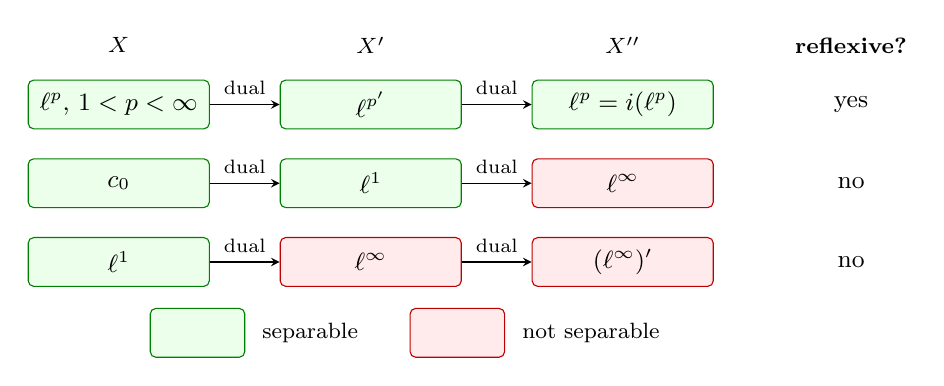
\begin{tikzpicture}[>=stealth, font=\small,
    sep/.style={draw=green!50!black, fill=green!8, rounded corners=2pt, minimum width=2.3cm, minimum height=0.62cm},
    non/.style={draw=red!75!black, fill=red!8, rounded corners=2pt, minimum width=2.3cm, minimum height=0.62cm}]
    \node[font=\footnotesize\bfseries] at (0,0.75) {$X$};
    \node[font=\footnotesize\bfseries] at (3.2,0.75) {$X'$};
    \node[font=\footnotesize\bfseries] at (6.4,0.75) {$X''$};
    \node[font=\footnotesize\bfseries] at (9.3,0.75) {reflexive?};
    \node[sep] (a1) at (0,0) {$\ell^p$, $1<p<\infty$};
    \node[sep] (a2) at (3.2,0) {$\ell^{p'}$};
    \node[sep] (a3) at (6.4,0) {$\ell^p = i(\ell^p)$};
    \node at (9.3,0) {yes};
    \node[sep] (b1) at (0,-1) {$c_0$};
    \node[sep] (b2) at (3.2,-1) {$\ell^1$};
    \node[non] (b3) at (6.4,-1) {$\ell^\infty$};
    \node at (9.3,-1) {no};
    \node[sep] (c1) at (0,-2) {$\ell^1$};
    \node[non] (c2) at (3.2,-2) {$\ell^\infty$};
    \node[non] (c3) at (6.4,-2) {$(\ell^\infty)'$};
    \node at (9.3,-2) {no};
    \foreach \r in {a,b,c} {
        \draw[->] (\r1) -- node[above, font=\scriptsize] {dual} (\r2);
        \draw[->] (\r2) -- node[above, font=\scriptsize] {dual} (\r3);
    }
    \node[sep, minimum width=1.2cm] at (1.0,-2.9) {};
    \node[right, font=\footnotesize] at (1.7,-2.9) {separable};
    \node[non, minimum width=1.2cm] at (4.3,-2.9) {};
    \node[right, font=\footnotesize] at (5.0,-2.9) {not separable};
\end{tikzpicture}
